%------------------------------------
% Début Partie Pierre
%------------------------------------
\part{Introduction}

\chapter{System prototype report}

\section{Abstract}
This project report will introduce you to the third year major group project. It will present all parts of the project, from the beginning with the research of an idea to the final product, through all steps. The final result is a computer's open source software called “QTypingTest“ usable on any platform (Window, Linux or Mac OS). The software is composed of different parts where users can learn how to type on a keyboard, improve what they have learned and use all this in a “competition” part. Users have access to statistics to show the evolution of their learning. The software has been developed using Qt, a cross-platform application software framework, which allows easy development of software that can be run on various platforms. 

\section{Introduction}
The application developed is a learning and testing software which gives users the opportunity to learn how to type well on a keyboard, to practice and to improve. When the software runs, the user is on the home page where they can create a new account and select or delete an existing one. Then, when an account is selected or created, the user has access to all different parts of the software. “Home” is used to send the user back to the home page, “Learn” is used to send the user to the section where they can learn how type. They can see which letters are learned and which ones need to be learned. “Practice” where the user has access to four different practice exercises, “Statistics” where the user can see statistics about their different practice and “Game” where they can find an interactive keyboard. 

\section{Brief walkthrough}
Basically, it is very simple to run the application. Indeed, the user just needs the executable (.exe) on their computer. When the software is running, the user can see the menu where they can select an existing user or create a new one and then navigate on the software. 

\section{Technology}
\begin{itemize}
    \item C++ is the language for this software.
    \item Qt (pronounced ‘Cute’ or ‘Q-T’) is a framework used to develop the software. It has been chosen because it is very suitable with C++ and to develop cross-platform software. The user does not need Qt on their computer to run the application. 
    \item Any software development platform (such as NetBeans or Eclipse …) could be used to code as long it supports Qt software. Qt company provides its own IDE, Qt Creator, which is very suitable because it includes some tutorials and the full library documentation of the framework. 
\end{itemize}

\section{Difficulties Faced}
The challenges faced were different for each member of the group. The principal one was at the beginning for both members of the group which was to understand how Qt was working because it was new for them. Pierre, also has some difficulties with C++ because he was less familiar with this language than Azarias. 

\section{Current Functionality}
\begin{itemize}
\item Can create a new user, use or delete an old one.
\item Users can use the "Learn" section and see the evolution of their learning.
\item Practice against time works.
\item Normal practice works.
\item Improve practice works.
\item Text practice works.
\item Users can see their own statistics.
\item Interactive keyboard.
\end{itemize}

\section{Next Stage Features}
\begin{itemize}
\item Translate the software to other languages
\item Develop a game
\item Allow competitions between users
\end{itemize}

\section{Conclusion}
The aim of this report is to cover all steps and to present all functionalities and choices the group made. The purpose is to produce a simple but robust and complete computer software. The final product, as presented, is fully functional and matches the group original idea.  

\chapter{Computing Domain}
The purpose if this project is to develop software so we adopted s suitable programming language for this. As the group members did C and Java in the first semester, we decided to use another one in a way to learn or to improve our skills on another language. This is why the group chose C++.
\\
C++ is a general object-oriented programming language which provides facilities with low-level memory manipulation. It was well adapted for our project because as C++ is a language which needs to be compiled, an executable is created and thereby can be used on user's computer to run the software. 
\\
There are different frameworks (libraries) available with C++ like Gtkmm, SFML or Qt for example. The group decided to use Qt because it was new for them and thus the project would give them a way to learn how to use it. Furthermore, Qt is well adapted for this type of software and the Qt company provides a good IDE (Qt Creator), which is fully working with the Qt library. This IDE provides a GUI builder and a documentation is directly included inside the IDE. 
\\
To build the design of the window's software, the group used the GUI builder provided buy Qt Creator.

\chapter{The project group}
The group consists two students. They realized that a gap of skill level existed and to be able to get a good final product, the group decide to try to find a way to split the work as equitably as possible, keeping in mind their objectives and personal skills.
\\
Azarias was working faster and getting more competence in C++ so he did more coding than Pierre. 
\\
C++ was new for Pierre so he had to adapt and make more time to learn the basics. 
\\
The report writing skills was pretty equals but as Pierre coded less he tried to spend more time as Azarias on this. 

\chapter{Project deliverables}
The deliverables as specified in the project handbook are:
\begin{itemize}
\item A working prototype.
\item An oral presentation and defence of the project.
\item System prototype documentation.
\item Full software.
\item A detailed project report.
\end{itemize}

\chapter{Document outline}
This report documentation presents the entire project from the beginning with the research to the final software.
All areas provided in this report are:
\begin{itemize}
\item An introduction, including a chapter containing a system prototype report, a chapter about the computing domain, a chapter about the project group, a chapter about the project deliverables and another with this document outline.
\item A complete literature review which covers the main research for the project. The different areas of research covered by this literature review are some historic research related to the subject, different keyboard available on the market and typing methods.  
\item A system analysis part containing a chapter covering different aspects of the functional requirements. 
\end{itemize}

\part{Literature review}
%\documentclass[12pt]{report}%??????autres?choix?:?book,?report
\usepackage[utf8]{inputenc}%???????????gestion?des?accents?(source)
\usepackage[T1]{fontenc}%??????????????gestion?des?accents?(PDF)
\usepackage[english]{babel}%english gestion
\usepackage{hyperref}
\usepackage[bottom]{footmisc}
\usepackage[font=small,labelfont=bf]{caption}
\usepackage[newparttoc]{titlesec}
\usepackage[nonumberlist,toc]{glossaries}
\usepackage[export]{adjustbox}
\usepackage[margin=0.95in]{geometry}
\usepackage[square,sort,comma,numbers]{natbib}

%All the packages
\usepackage{lmodern,url,ragged2e,textcomp,lmodern,paralist}
\usepackage{graphicx,xcolor,float,afterpage}
\usepackage{chngcntr,csquotes,helvet,lastpage}
\usepackage{subcaption,wrapfig,fancyhdr,blindtext}
\usepackage{titletoc,transparent,datatool}

%List de mot ordonné
\newcommand{\sortitem}[1]{%
  \DTLnewrow{list}% Create a new entry
  \DTLnewdbentry{list}{description}{#1}% Add entry as description
}
\newenvironment{sortedlist}{%
  \DTLifdbexists{list}{\DTLcleardb{list}}{\DTLnewdb{list}}% Create new/discard old list
}{%
  \DTLsort{description}{list}% Sort list
  \begin{center}
	  \begin{inparaitem}%
    		\DTLforeach*{list}{\theDesc=description}{%
         \item \theDesc \hspace{0.1cm} }% Print each item
      \end{inparaitem}•%  
  \end{center}
}

%Nouvelles commandes
\renewcommand{\familydefault}{\sfdefault} %default font
\newcommand{\HRule}{\rule{\linewidth}{0.5mm}}
\newcommand{\Mline}{\hrule \mbox{}\\[0.1cm]}
\renewcommand{\thechapter}{\Roman{chapter}}

%final last page
\newcommand\blankpage{%
    \null
    \thispagestyle{empty}%
    \addtocounter{page}{-1}%
    \newpage}


%FORMAT DU CHAPITRE
\titleclass{\chapter}{straight}
\titleformat{\chapter}[hang]
  {}
  {\normalfont \sffamily \bfseries \thechapter.}
  {0pt}
  {\normalfont \sffamily \bfseries}
\titlespacing*{\chapter}{0pt}{50pt}{18pt}

%FORMAT De section
\renewcommand*\thesection{\arabic{section}}
\titleclass{\section}{straight}
\titleformat{\section}[hang]
  {}
  {\small \sffamily \bfseries \textit \thesection . }
  {0pt}
  {\small \bfseries \textit}
  
\titlespacing*{\chapter}{0pt}{50pt}{18pt}

%Comptage des figures
\renewcommand{\thefigure}{\arabic{figure}}

%Ne pas reset le numéro des figures  à chaque chapitre
\counterwithout{figure}{chapter}

%Custom footer and header
\pagestyle{fancy}
\fancyhf{}
%\lhead{Implement a Typing Speed Test With Qt}
\rhead{B00092351 Azarias Boutin, B00092354 Pierre Thubé}
\rfoot{Page \thepage}

\begin{document}

\begin{titlepage}
\begin{center}


% Title
\Mline
{ \LARGE Implement a Typing Speed Test With Qt \\[0.4cm] }
{ \LARGE Literature Review\\[0.4cm] }
\Mline
% Author and supervisor

\textsf{}\\[3cm]

\textsf{Boutin Azarias B00092351, B00092354 Pierre Thubé - Group 2\\[2cm]
BN013 BSC in Computing}


\end{center}
\end{titlepage}
\clearpage

\tableofcontents
\listoffigures
\chapter*{Keywords}
\begin{sortedlist}
  \sortitem{Keyboard}
  \sortitem{Keyboard layout}
  \sortitem{Fingers}
  \sortitem{Keys}
  \sortitem{Speed}
  \sortitem{Accuracy}
  \sortitem{Typing}
  \sortitem{Improvements}
  \sortitem{Learning}
\end{sortedlist}

\thispagestyle{empty}
\clearpage

\setcounter{page}{1}
\chapter{Abstract}
This review explores the way of improving the typing speed on the common keyboard.
Today's world is already full of keyboards, and it will never cease to increase. To be more efficient when using a computer, it is a good idea to learn how to type. On the web there are plenty of sources to improve your skills, but there is very little of them who really teach you how to type faster from scratch. The same goes for the existing software. And the main issue regarding this is that the software is not free.\\
The work presented here is based on books and websites that give advice on how to type speedily.\\
In order to address that issue, this review looks at the finger positions. Then it goes on to discuss how the user must practice to improve his or her typing skills. Lastly, it looks at the importance of accuracy and how this outweighs speed.

\clearpage
\chapter{Literature review}
\section{Some history}
In 1890, Lovisa Ellen Barnes wrote a book called "How To Become Expert in Typewriting"\cite{ref2} who was explaining how type on a Remington Typewriter.\\
In 1915, Dr. Henry Faulds wrote a book called "A Manual of Practical Dactylography"\cite{ref3}\\
An other example of book talking about dactylography.\cite{ref5}\\   
A more recent one published in 2012 and wrote by Faulds H.\cite{ref4}\\
As we can see, from a long time people provide way to learn how type so we can thereby say that way to type, and so typing speed, are always being important and are never been neglect by people.\\

\section{Keyboard}
The original layouts for the first mechanical typewriters were in alphabetical order (ABCDE etc..). Then different type of keyboard appeared according to languages used in each country (the most used is the QWERTY one but you can find AZERTY in France or QWERTZ in Germany for example).\\
Each of this layouts keyboard are classics one, that is mean when you buy a keyboard you will have one of this, but, since the invention of computers and indeed keyboards, a lots of research 	conducted to the invention of new non-classics layouts. Indeed, this new layouts had to made typing more easy and more comfortable. The most famous are Dvorak, Colemak and Workman.\\
Dvorak has been invented by August Dvorak and is the best alternative to QWERTY. It has been designed to increase typing speed, decrease errors and increase comfort.\\
After Dvorak, Colemak is the most popular. Also based on the QWERTY keyboard, it has been created in 2006 by Shai Coleman. It allow to promote the bearing of fingers on the middle rows of keys, it is better to maximise alternation between use right and left hands and minimize the movement of hands on the keyboard.\\
The third one is Workman. Thise one is less used than Dvorak and Colemak, but according with different developers, it is actually the best one to reduce fingers exhaustion. Indeed, it reduce usage of the two middle columns, reduce horizontal,diagonal and vertical finger stretching compared to Dvorak and Colemak.\cite{ref6}\\
To conclude about that, we can obviously say that from people have always trying to increase their typing skills by inventing new keyboards layouts which increase typing comfort and thus typing speed.     
\begin{figure}[h!]
   \begin{minipage}[b]{0.32\linewidth}
      \centering 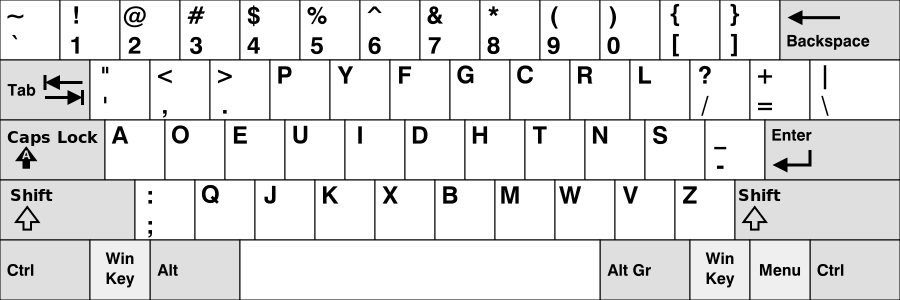
\includegraphics[scale=0.16]{images/KB_United_States_Dvorak.png}
      \caption{\it Dvorak Keyboard}
   \end{minipage}
   \begin{minipage}[b]{0.32\linewidth}   
      \centering 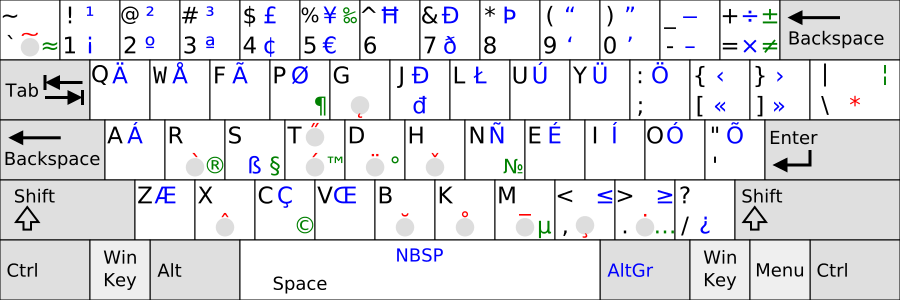
\includegraphics[scale=0.16]{images/KB_US-Colemak_with_AltGr.png}
      \caption{\it Colemak Keyboard}
   \end{minipage}
   \begin{minipage}[b]{0.32\linewidth}
      \centering 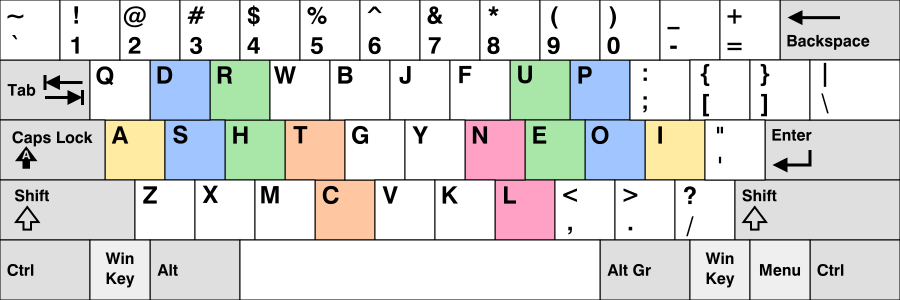
\includegraphics[scale=0.16]{images/KB_English_Workman.png}
      \caption{\it Workman Keyboard}
   \end{minipage}
\end{figure}
\clearpage

\section{Typing way and Fingers position}
To improve typing speed, in addition to change our keyboard, the only way is to practice. Actually, the average typing speed, calculate in Word Per Minute (WPM), is of 44 words.\cite{ref7} In the English language, the fastest typist in the world was Stella Pajunas who had a top speed of 216 words per minute. She realize it on a typewriter in 1946. Nowadays, it is easy with practice to had a typing speed of about 100 words par minute.\\ 
The typing way, which can be learn and improve on a lots of software and websites, is really the most important things to take in consideration to improve our typing speed. This typing way include the position of hands on a keyboard, which will change according to the type of keyboard, but for a QWERTY one it is like the figure 4 shows.
\begin{figure}[H]
\begin{center}
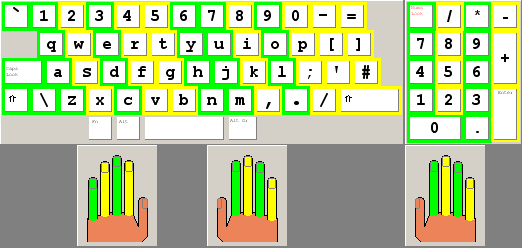
\includegraphics[width=9cm]{images/FingerHandPosUSA.png} 
\end{center}
\caption{\it Fingers position on QWERTY keyboard}
\label{Poulpy est multicolore}
\end{figure}
Here you can find some example of typing test on the internet:
\begin{itemize}
\item\it TypingTest.com\cite{ref8}
\item\it 10fastfingers.com\cite{ref9}
\end{itemize}
It also possible to find typing lessons on the internet.\\
To conclude about this part we can say that way to type and typing speed are things very democratize on the internet especially with a lots of website who can explain you best way to type, position of hands, give you advice and way to improve your typing style with speed test. That is showing that the development of a typing test is something useful.
Every book and website available regarding improving the typing speed are first mentions the finger positions.\\
As the book written by \citet{beginners}, the fingers must be positioned on the \textit{baseline}. The baseline, is the line on the keyboard containing the letters \textit{F} and \textit{J}. As with 'touch typing in ten lessons' \cite{tenlessons} book explains, every fingers should have an assigned letter. The figure below \ref{fing_pos} shows where the finger position is assigned on a QWERTY keyboard.
\begin{figure}[H]
	\centering
	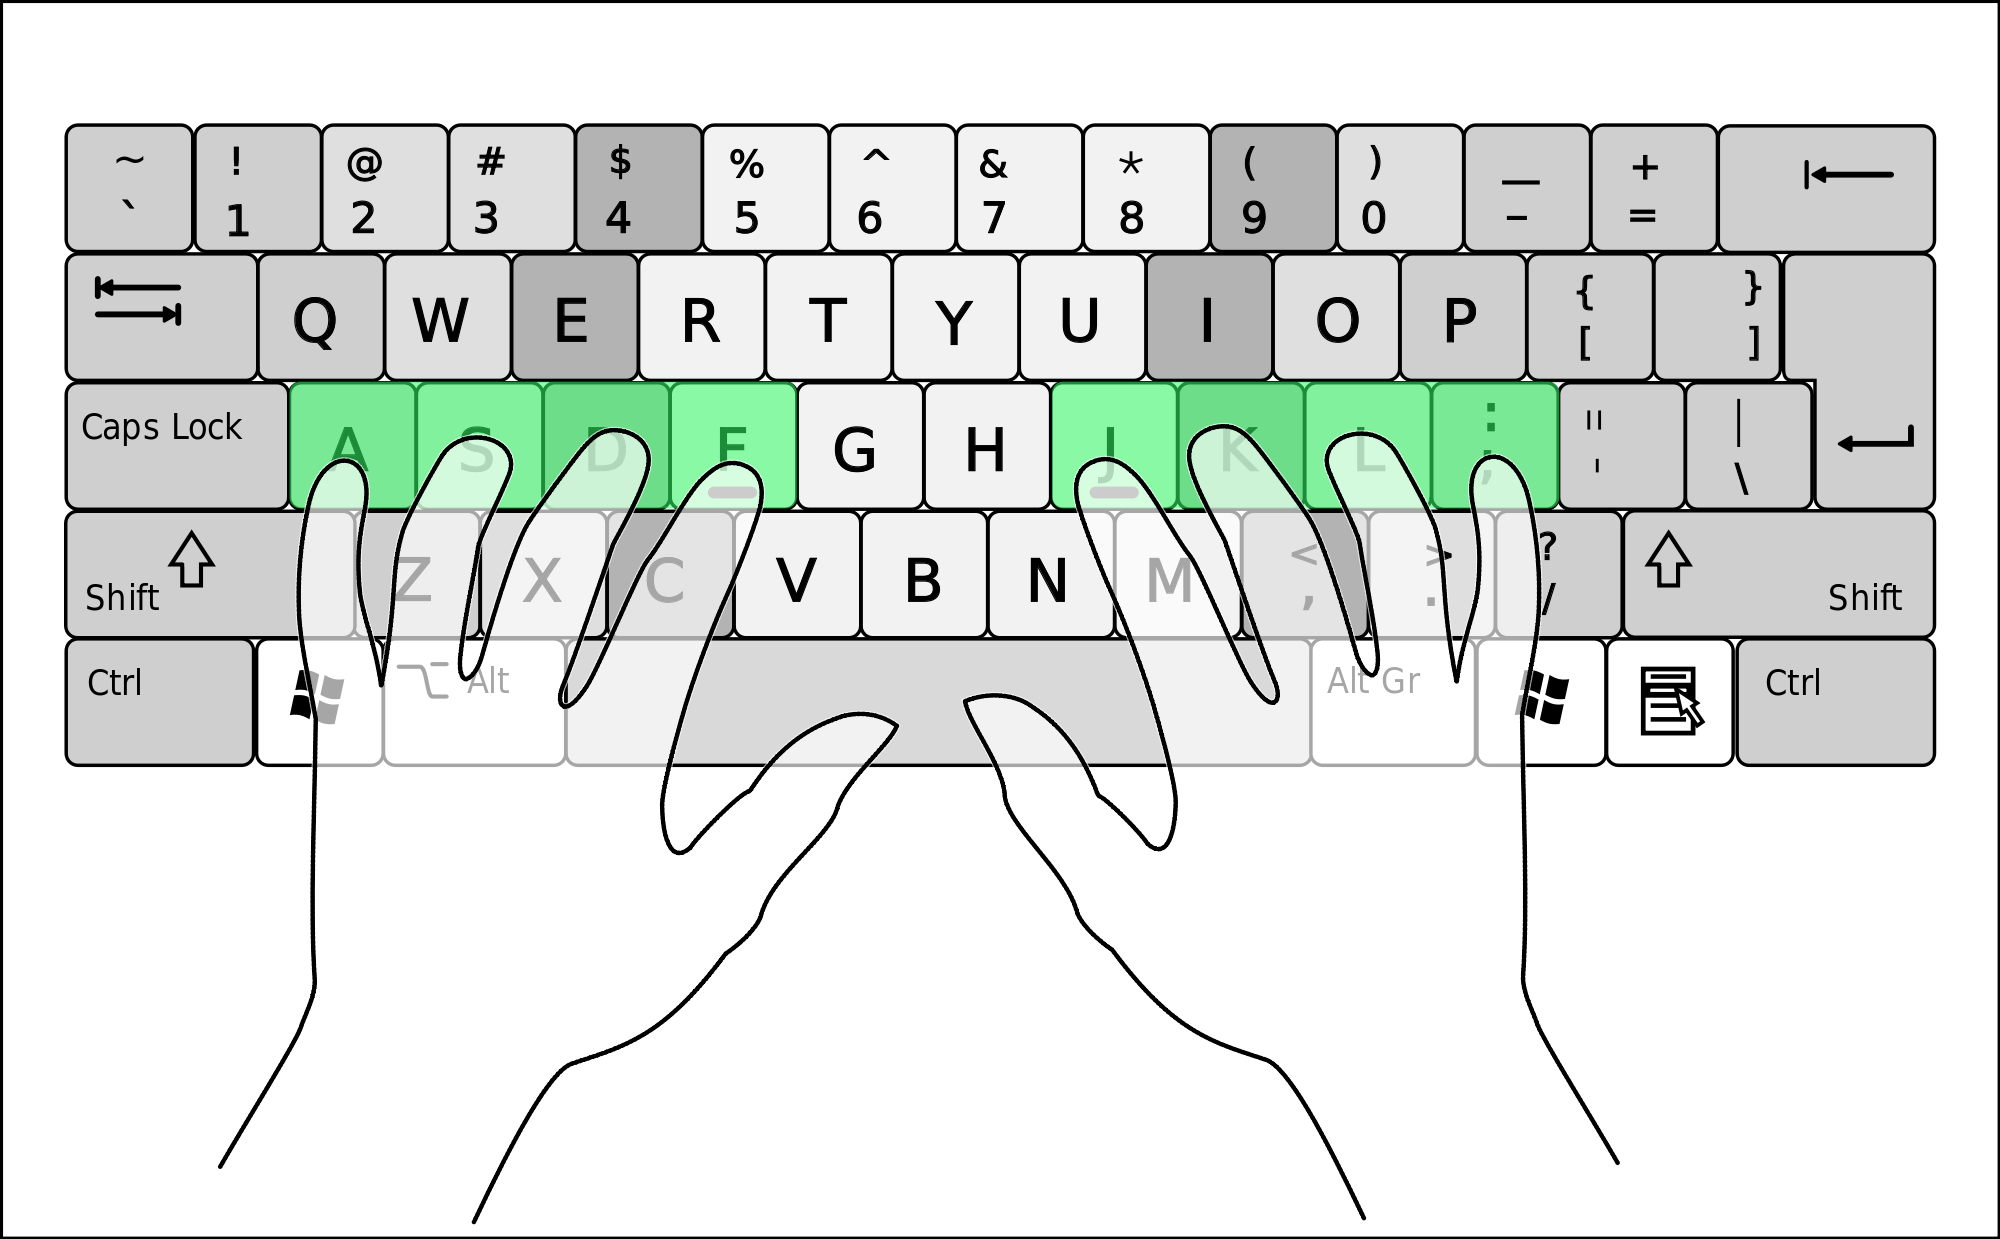
\includegraphics[width=0.7\textwidth]{images/fing_pos.png}
	\caption{Position of the fingers on a QWERTY keyboard}\label{fing_pos}
\end{figure}
However, the layout of the keyboard may vary but the finger position will stay on the same baseline. www.computerhope.com \cite{computerhope} shows the different keys for each finger depending on the keyboard layout.
Other keyboards exist such as those represented in 'typing for beginners' \citep{beginners}. Unfortunately there are not common enough and are only used by more professional typists. So this literature review will not cover the use of them.\\
The user must know which finger is assigned to its specific letter on the keyboard. And so forth for each row. The book written by
\citet{beginners} explains the differents steps on how to follow the assignment for each row. Once again, the letters may vary depending on the keyboard layout, but the finger movements are still the same.
\begin{figure}[H]
    \centering
    \begin{subfigure}[b]{0.3\textwidth}
        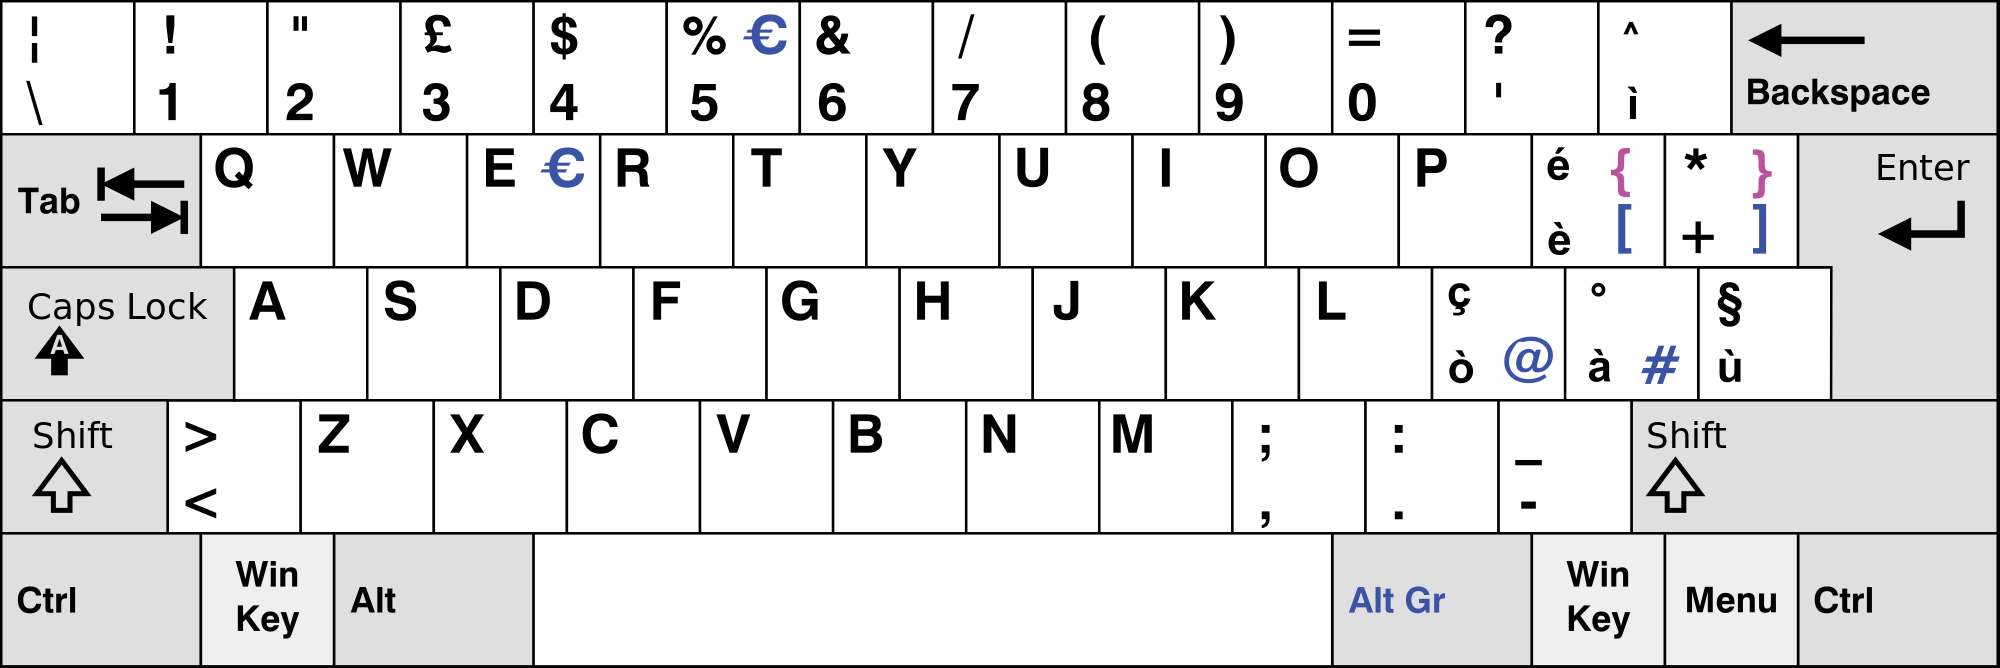
\includegraphics[width=\textwidth]{images/qwerty.png}
        \caption{Qwerty-based layout}
    \end{subfigure}
	 \begin{subfigure}[b]{0.3\textwidth}
        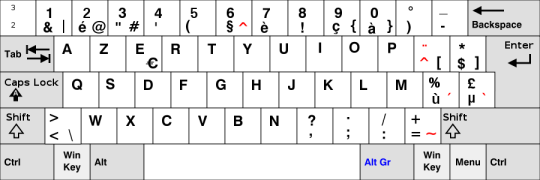
\includegraphics[width=\textwidth]{images/azerty.png}
        \caption{Azerty-based layout}
    \end{subfigure} 
    \begin{subfigure}[b]{0.3\textwidth}
        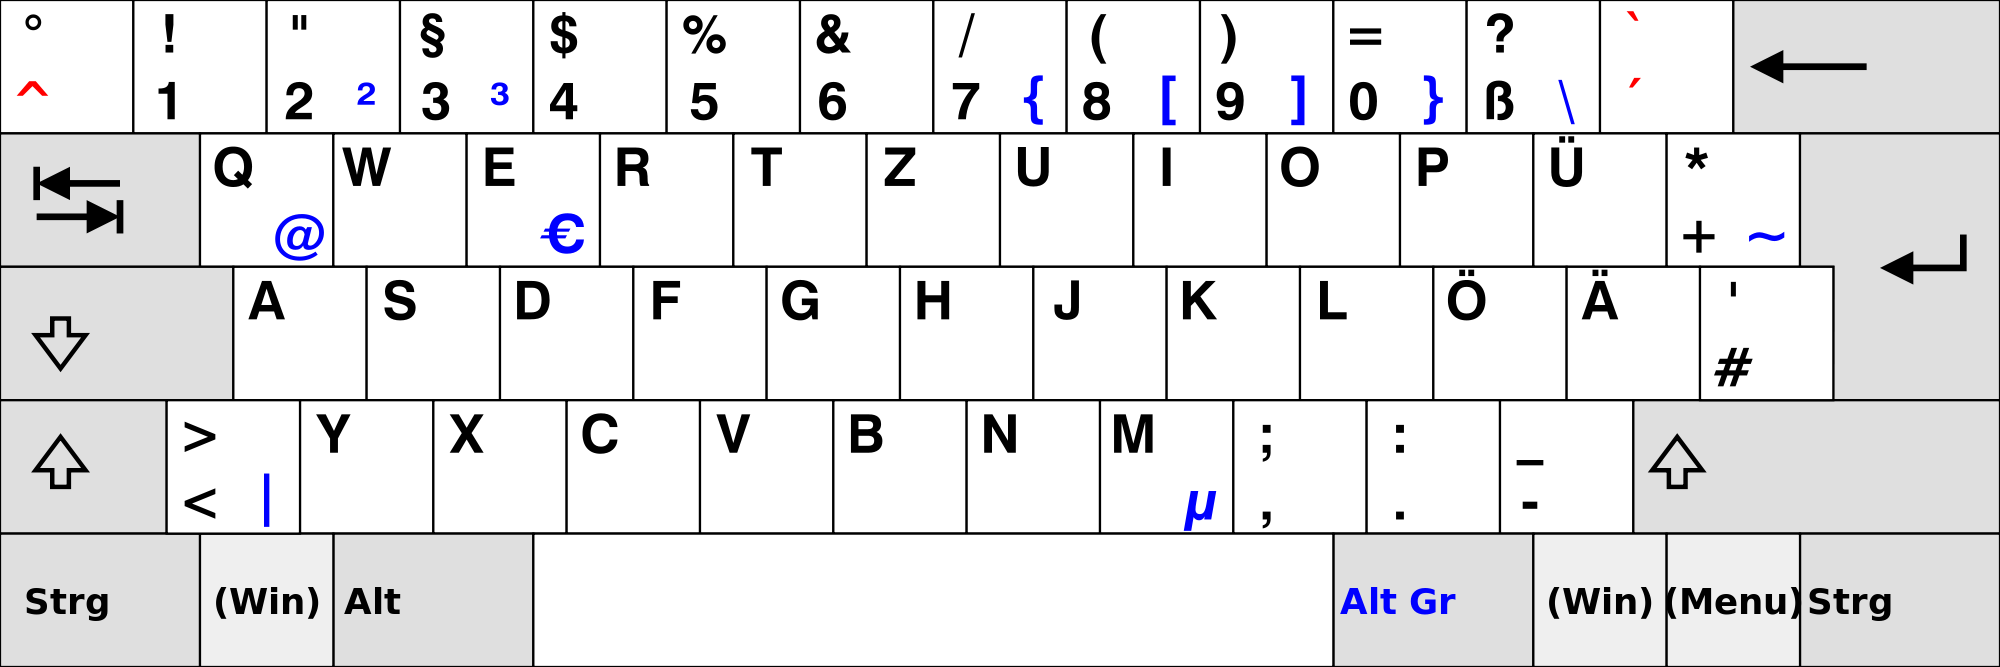
\includegraphics[width=\textwidth]{images/qwertz.png}
        \caption{Qwertz-based layout}
    \end{subfigure}
    \caption{Most common layouts in Europe}
\end{figure}
\clearpage

\section{Practice}
The more you know, the more you type. Once you are able to type a full word one needs to keep practising. This builds up a muscle memory of all the possible key stokes which make up the words of the dictionary.
The computerhope.com\citep{computerhope} website provide good everyday practice example to follow. There is also a large collection of games on the internet to practice and therefore improve the typing speed.\\
how-to-type.com \cite{howto} offers practice sessions such as 10 minutes to an hour per session as their recommendation.
The book written by \citet{handBook} also gives some advice regarding the finger position and the stretch to do beforehand.
There is no software which combines both, doing a check that the user has done finger stretches, and provide advice on how to position yourself in front of the keyboard improving your ability to type correctly. Each of these is done on an individual basis.

\section{Speed and accuracy}
Accuracy is the first skill we need to develop (typing for beginners)\cite{beginners}.\\
Firstly, the user must learn how to type all the letters of the keyboard, as said above. The user must know the exact position of each letter on the keyboard, without having to look at it. Once they know this, they will have the ability to type much faster. However faster can also mean more mistakes. If the mistake is found on the same letter, the user must practice typing this letter again and again to improve accuracy. The problem can also come from a finger which is not reactive enough. In this case, steps need to be put in place in order to train that particular finger. This will be one of the goals of the software to be created. Also, the user must be aware that the more improvement regarding typing speed, the harder it will become to improve this speed.(lingholic.com) \cite{plateau}. Below are two graphs explaining the difference between the expected learning curve and the actual learning curve.

\begin{figure}[H]
    \centering
    \begin{subfigure}[b]{0.4\textwidth}
        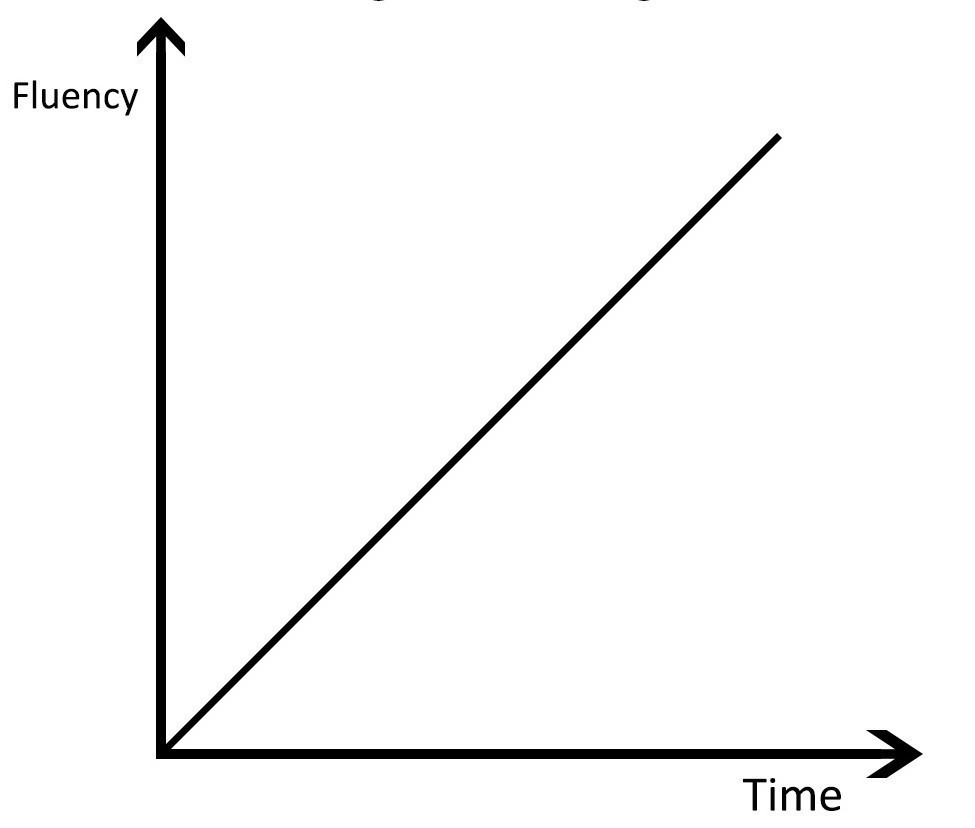
\includegraphics[width=\textwidth]{images/expected.jpg}
        \caption{Expected learning curve}
    \end{subfigure}
    \begin{subfigure}[b]{0.4\textwidth}
        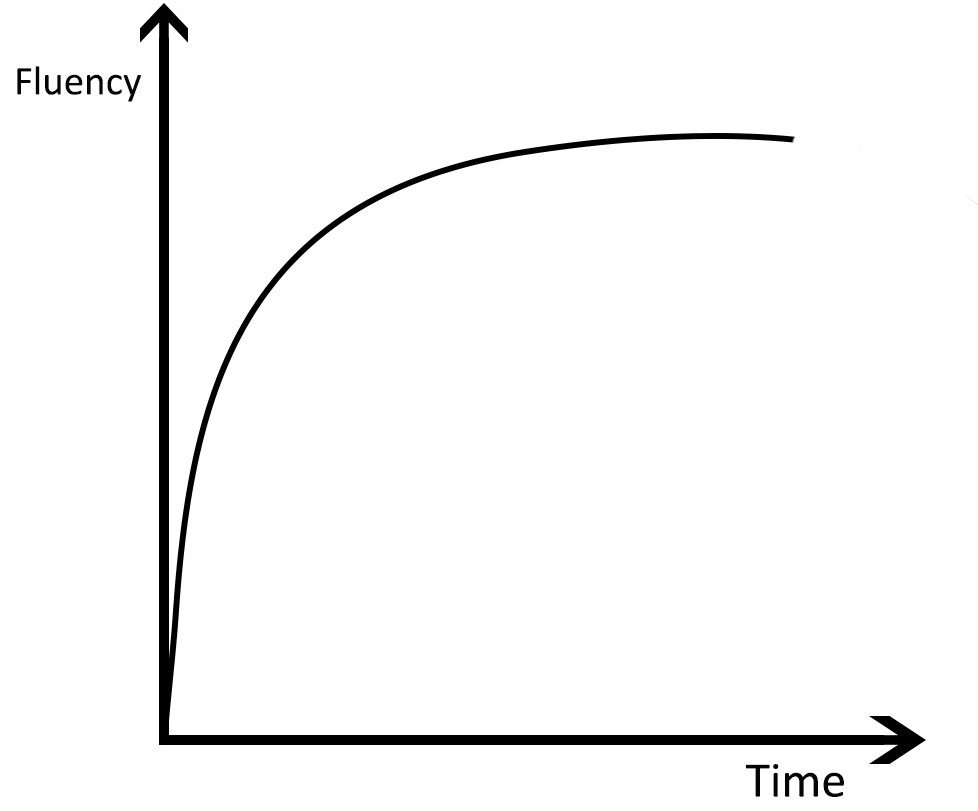
\includegraphics[width=\textwidth]{images/actual.jpg}
        \caption{Actual learning curve}
    \end{subfigure}
    \caption{Expected and actual learning curve}
\end{figure}

\clearpage
\chapter{Conclusion}
From the current knowledge in typing, it appears that it is possible to quickly easily to learn to type faster and with a good accuracy. It is important for the user to learn the basics of the keyboard and the position of the letters. Once this is known, with the time and practice, typing speed will slowly and steadily increase.\\
Whenever the user has some accuracy problem with a single finger, practice will increase general precision.\\
For the general public, it they have a computer and a keyboard, they can learn how to type faster in three steps :
\begin{itemize}
	\item Learn the position of the letters on the keyboard and associate each fingers to each key
	\item Practice in order to improve the speed
	\item Correct the accuracy problems
\end{itemize}

\clearpage

%Bibliography
\begin{flushleft}
	\bibliographystyle{unsrtnat}
	\bibliography{lit_review.bib}
\end{flushleft}

\clearpage
\afterpage{\blankpage}

\end{document}
\chapter*{Keywords}
\begin{sortedlist}
  \sortitem{Keyboard}
  \sortitem{Keyboard layout}
  \sortitem{Fingers}
  \sortitem{Keys}
  \sortitem{Speed}
  \sortitem{Accuracy}
  \sortitem{Typing}
  \sortitem{Improvements}
  \sortitem{Learning}
\end{sortedlist}


\chapter{Abstract}
This review explores the way of improving the typing speed on the common keyboard.
Today's world is already full of keyboards, and it will never cease to increase. To be more efficient when using a computer, it is a good idea to learn how to type. On the web there are plenty of sources to improve your skills, but there are very few of them that really teach you how to type faster from scratch. The same goes for the existing software and the main issue regarding this is that the software is not free.\\
The work presented here is based on books and websites that give advice on how to type speedily.\\
In order to address that issue, this review looks at the finger positions. Secondly, it goes on to discuss how the user must practice to improve his or her typing skills. Lastly, it looks at the importance of accuracy and how this outweighs speed.

\clearpage
\chapter{Literature review}
\section{Some history}
In 1890, Lovisa Ellen Barnes wrote a book called "How To Become Expert in Typewriting"\cite{ref2} who was explaining how type on a Remington Typewriter.\\
In 1915, Dr. Henry Faulds wrote a book called "A Manual of Practical Dactylography"\cite{ref3}\\
An other example of book talking about dactylography.\cite{ref5}\\   
A more recent one published in 2012 and wrote by Faulds H.\cite{ref4}\\
As we can see, for a long time people provided ways to learn how type. Thereby we can say that way to type has always been important not neglected by people.\\

\section{Keyboard}
The original layout for the first mechanical typewriters were in alphabetical order (ABCDE etc..). Then different types of keyboards appeared according to language used in each country (the most used is the QWERTY one but you can find AZERTY in France or QWERTZ in Germany for example).\\
Each of these keyboard layouts are classics ones, meaning when you buy a keyboard you will have one of these. Since the invention of computers and indeed keyboards, lots of research has been conducted regarding the invention of new non-classics keyboard layouts. Indeed, these new styles have made typing more easy and more comfortable. The most famous are Dvorak, Colemak and Workman.\\
Dvorak has been invented by August Dvorak and is the best alternative to QWERTY. It has been designed to increase typing speed, decrease errors and increase comfort.\\
After Dvorak, Colemak is the most popular. Also based on the QWERTY keyboard, it has been created in 2006 by Shai Coleman. It promotes the bearing of fingers on the middle rows of keys, it is better to maximise alternation between the use of right and left hands and minimizes the movement of hands on the keyboard.\\
The third one is Workman. This one is less used than Dvorak and Colemak, but according to different developers, it is actually the best one to reduce finger exhaustion. Indeed, it reduces usage of the two middle columns, reduces horizontal,diagonal and vertical finger stretching compared to Dvorak and Colemak.\cite{ref6}\\
To conclude, we can say that people have always tried to increase their typing skills by inventing new keyboard layout which increase typing comfort and thus typing speed.     
\begin{figure}[h!]
   \begin{minipage}[b]{0.32\linewidth}
      \centering 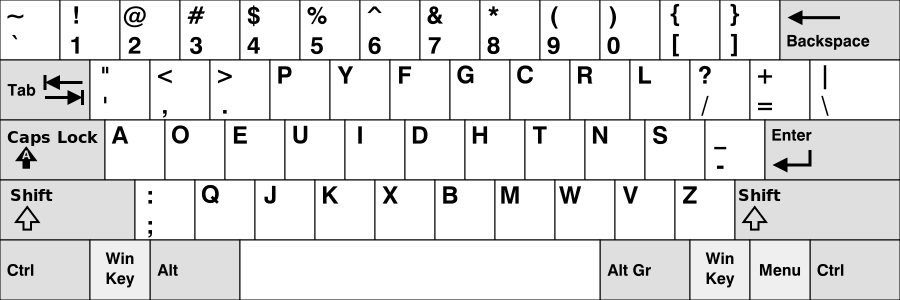
\includegraphics[scale=0.16]{images/KB_United_States_Dvorak.png}
      \caption{\it Dvorak Keyboard}
   \end{minipage}
   \begin{minipage}[b]{0.32\linewidth}   
      \centering 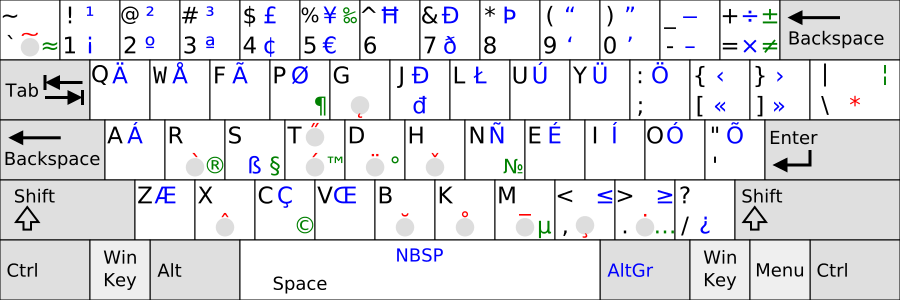
\includegraphics[scale=0.16]{images/KB_US-Colemak_with_AltGr.png}
      \caption{\it Colemak Keyboard}
   \end{minipage}
   \begin{minipage}[b]{0.32\linewidth}
      \centering 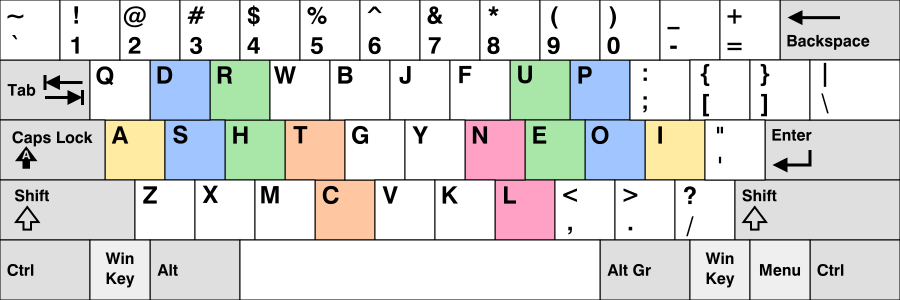
\includegraphics[scale=0.16]{images/KB_English_Workman.png}
      \caption{\it Workman Keyboard}
   \end{minipage}
\end{figure}

\section{Typing method and Finger position}
To improve typing speed, in addition to changing the keyboard, the only way is with practice. Actually, the average typing speed, calculated in Word Per Minute (WPM), is of 44 words.\cite{ref7} In the English language, the fastest typist in the world was Stella Pajunas who had a top speed of 216 words per minute. She realize it on a typewriter in 1946. Nowadays, it is easy with practice to have a typing speed of about 100 words per minute.\\ 
The typing way, which can be learned and improved on lots of software and websites, is really the most important thing to take in consideration to improve our typing speed. This typing way includes the position of hands on a keyboard, which will change according to the type of keyboard, but for a QWERTY one it is as figure 4 shows.
\begin{figure}[H]
\begin{center}
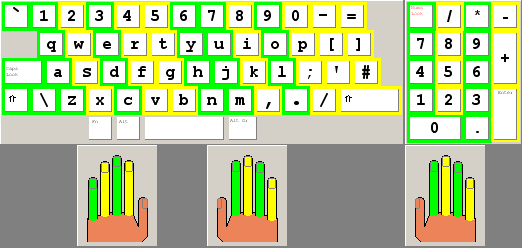
\includegraphics[width=9cm]{images/FingerHandPosUSA.png} 
\end{center}
\caption{\it Fingers position on QWERTY keyboard}
\label{Poulpy est multicolore}
\end{figure}
Here you can find some example of typing test on the internet:
\begin{itemize}
\item\it TypingTest.com\cite{ref8}
\item\it 10fastfingers.com\cite{ref9}
\end{itemize}
It also possible to find typing lessons on the internet.\\
To conclude this part we can say that the way to type and typing speed are documented on the internet, with lots of websites explaining the best way to type, position of hands, give advice and ways to improve your typing style with speed tests. This demonstrates that the development of a typing test is something useful.
Every book and website available regarding improving the typing speed first mentions the finger position.\\
As the book written by \cite{beginners}, the fingers must be positioned on the \textit{baseline}. The baseline, is the line on the keyboard containing the letters \textit{F} and \textit{J}. As with 'touch typing in ten lessons' \cite{tenlessons} book explains, every finger should have an assigned letter. The figure below \ref{fing_pos} shows where the finger position is assigned on a QWERTY keyboard.
\begin{figure}[H]
	\centering
	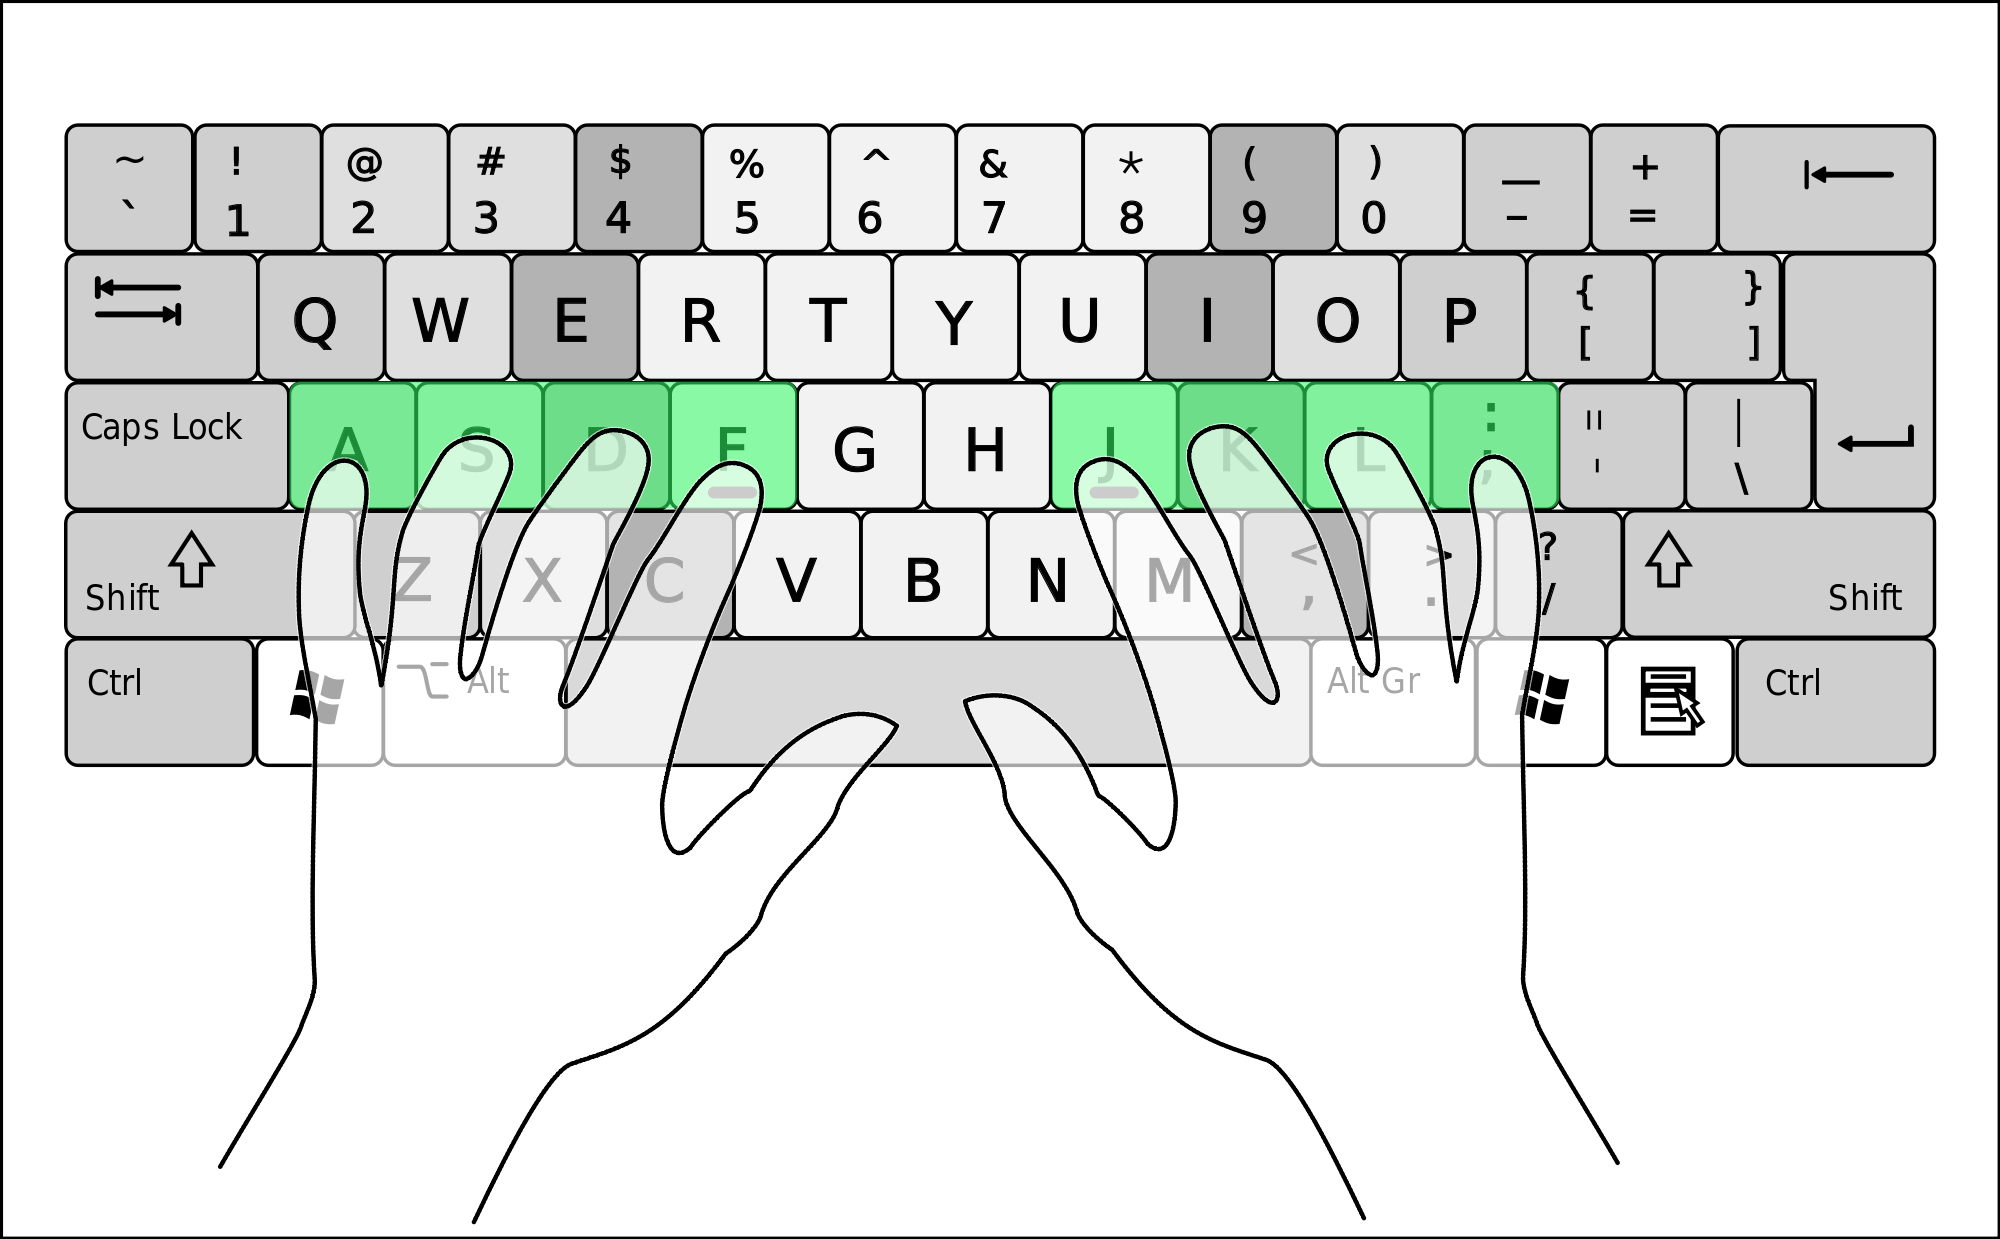
\includegraphics[width=0.7\textwidth]{images/fing_pos.png}
	\caption{Position of the fingers on a QWERTY keyboard}\label{fing_pos}
\end{figure}
However, the layout of the keyboard may vary but the finger position will stay on the same baseline. www.computerhope.com \cite{computerhope} shows the different keys for each finger depending on the keyboard layout.
Other keyboards exist such as those represented in 'typing for beginners' \cite{beginners}. Unfortunately they are not common enough and are only used by professional typists. So this literature review will not cover the use of them.\\
The user must know which finger is assigned to its specific letter on the keyboard. And so forth for each row. The book written by \cite{beginners} explains the different steps on how to follow the assignment for each row. Once again, the letters may vary depending on the keyboard layout, but the finger movements are still the same.
\begin{figure}[H]
    \centering
    \begin{subfigure}[b]{0.3\textwidth}
        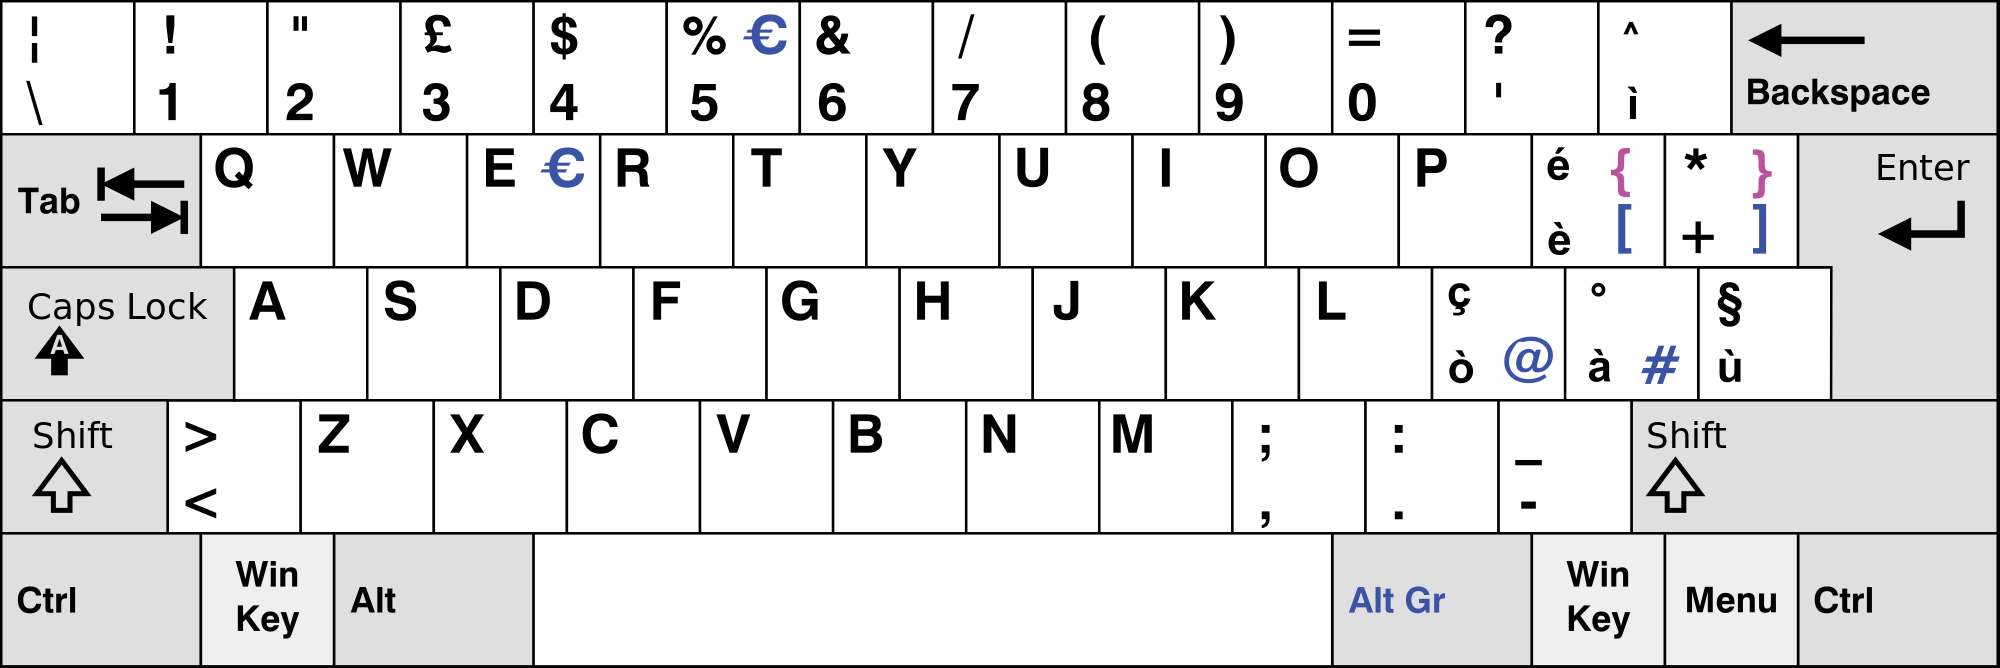
\includegraphics[width=\textwidth]{images/qwerty.png}
        \caption{Qwerty-based layout}
    \end{subfigure}
	 \begin{subfigure}[b]{0.3\textwidth}
        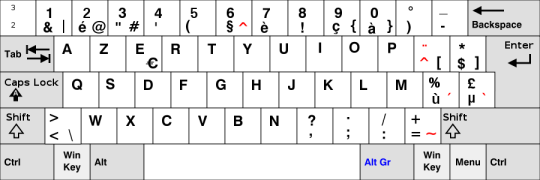
\includegraphics[width=\textwidth]{images/azerty.png}
        \caption{Azerty-based layout}
    \end{subfigure} 
    \begin{subfigure}[b]{0.3\textwidth}
        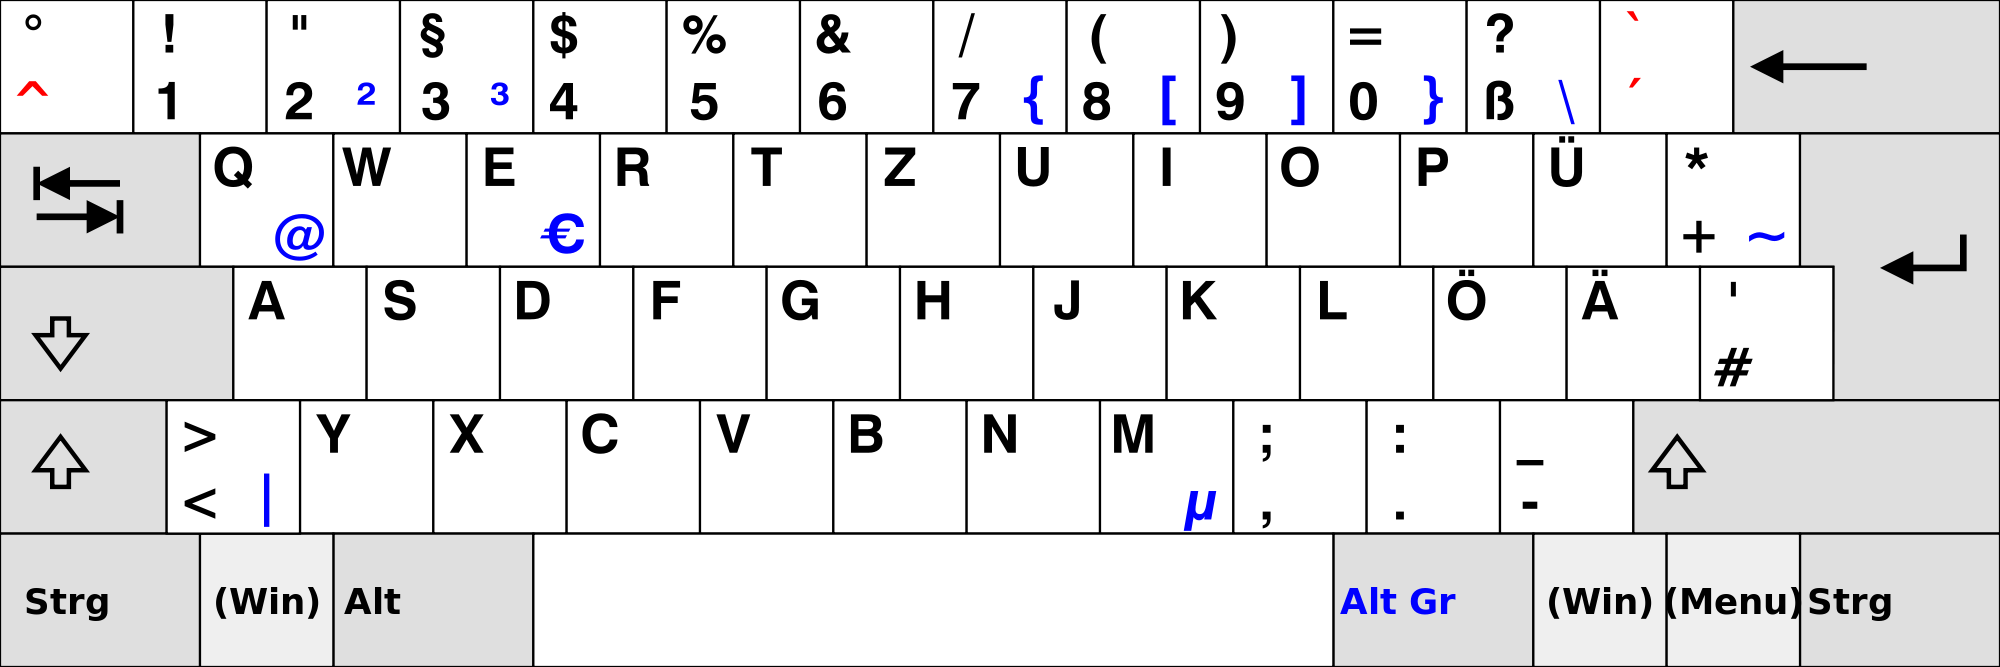
\includegraphics[width=\textwidth]{images/qwertz.png}
        \caption{Qwertz-based layout}
    \end{subfigure}
    \caption{Most common layouts in Europe}
\end{figure}

\section{Practice}
The more you know, the more you type. Once you are able to type a full word one needs to keep practising. This builds up a muscle memory of all the possible key stokes which make up the words of the dictionary.
The computerhope.com\cite{computerhope} website provide good everyday practice examples to follow. There is also a large collection of games on the internet to practice and therefore improve the typing speed.\\
how-to-type.com \cite{howto} offers practice sessions such as 10 minutes to an hour per session as their recommendation.
The book written by \cite{handBook} also gives some advice regarding the finger position and the stretch to do beforehand.
There is no software which combines both, doing a check that the user has done finger stretches, and provide advice on how to position yourself in front of the keyboard improving your ability to type correctly. Each of these is done on an individual basis.

\section{Speed and accuracy}
Accuracy is the first skill we need to develop (typing for beginners)\cite{beginners}.\\
Firstly, the user must learn how to type all the letters of the keyboard, as outlined above. The user must know the exact position of each letter on the keyboard, without having to look at it. Once they know this, they will have the ability to type much faster. However faster can also mean more mistakes. If the mistake is found on the same letter, the user must practice typing this letter again and again to improve accuracy. The problem can also come from a finger which is not reactive enough. In this case, steps need to be put in place in order to train that particular finger. This will be one of the goals of the software to be created. Also, the user must be aware that the more improvement regarding typing speed, the harder it will become to improve this speed.(lingholic.com) \cite{plateau}. Below are two graphs explaining the difference between the expected learning curve and the actual learning curve.

\begin{figure}[H]
    \centering
    \begin{subfigure}[b]{0.4\textwidth}
        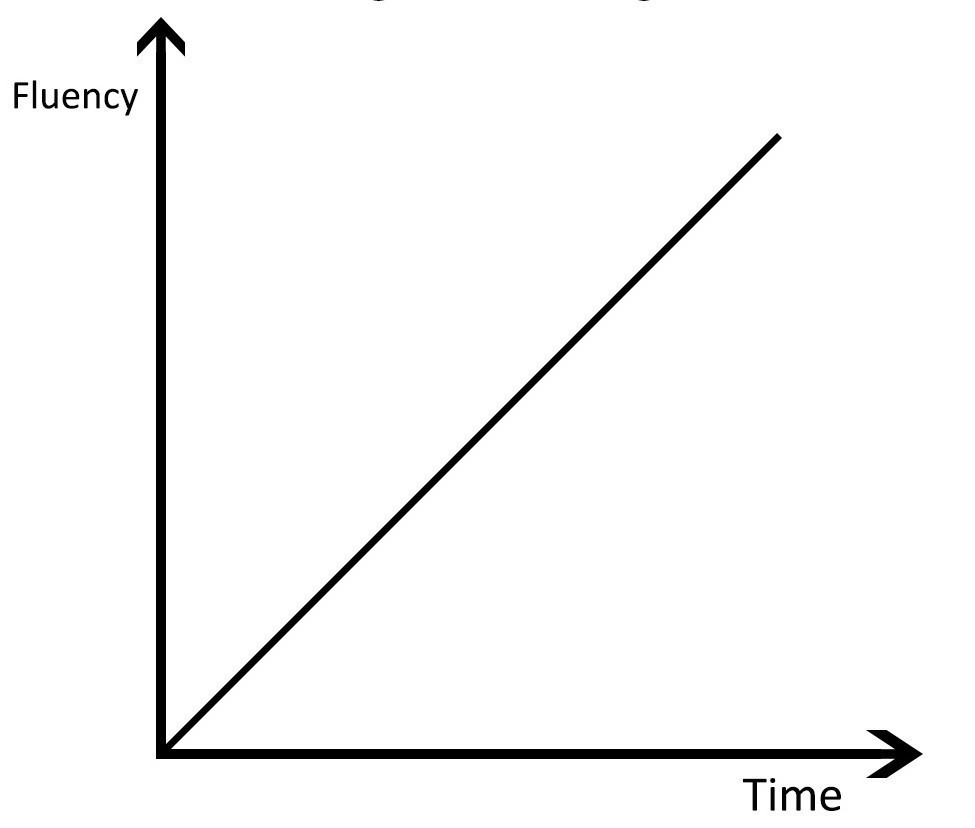
\includegraphics[width=\textwidth]{images/expected.jpg}
        \caption{Expected learning curve}
    \end{subfigure}
    \begin{subfigure}[b]{0.4\textwidth}
        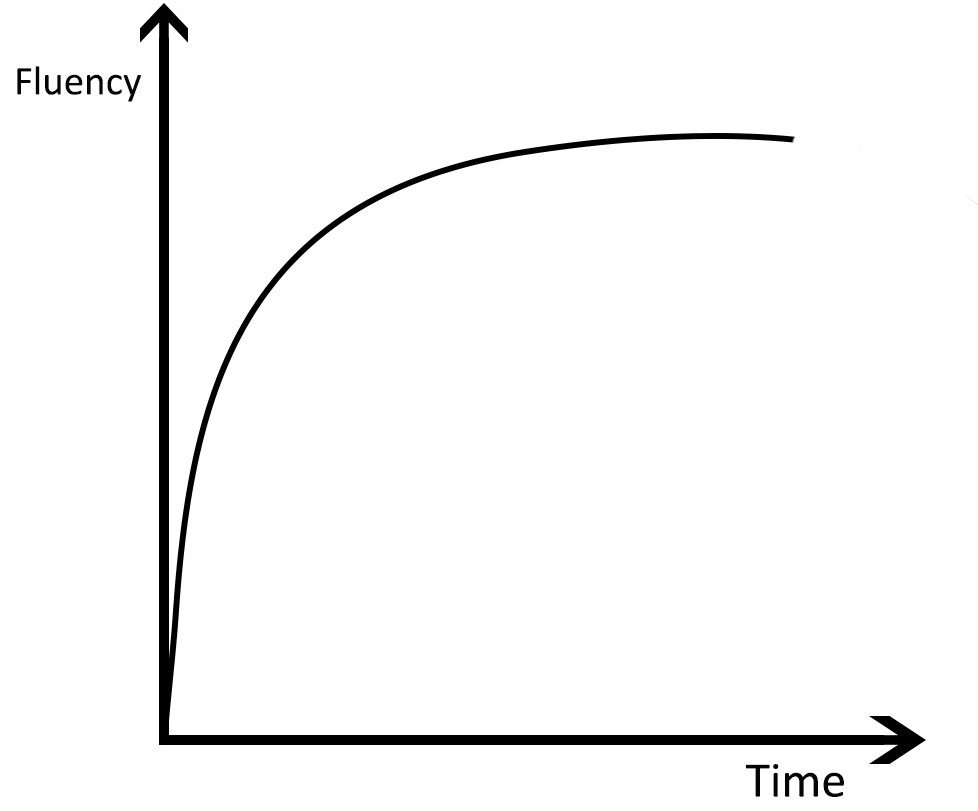
\includegraphics[width=\textwidth]{images/actual.jpg}
        \caption{Actual learning curve}
    \end{subfigure}
    \caption{Expected and actual learning curve}
\end{figure}

\chapter{Conclusion}
From current knowledge in typing, it appears that it is possible to quickly and easily learn to type faster and with good accuracy. It is important for the user to learn the basics of the keyboard and the position of the letters. Once this is known, with time and practice, typing speed will slowly and steadily increase.\\
Whenever the user has some accuracy problem with a single finger, practice will increase general precision.\\
In general, if a person has a computer and a keyboard, they can learn how to type faster in three steps :
\begin{itemize}
	\item Learn the position of the letters on the keyboard and associate a finger to each key
	\item Practice in order to improve speed
	\item Correct accuracy problems
\end{itemize}

%Bibliography
\begin{flushleft}
	\bibliographystyle{plain}
	\bibliography{lit_review}
\end{flushleft}

\part{System analysis}

\chapter{Functional requirements}
C++an provide users executable file which is the only thing they need to run the software on their computer.

\section{What the software does}
This application is a learning and testing software using Qt framework and developed with C++ language. The software provides a way for users to learn from the beginning how type fast and accurately on a keyboard.
\\
The learning part is divided in forty-eight sections ("Learn" part in the GUI), each one gives the user training for different groups of letters. At the beginning when the user account is new, only the first training is available. When a user selects a training group of letters, a keyboard layout is displayed (depending on the layout the user selects in their parameters) explaining where the letters are on the keyboard and which fingers are used. The first group is "fj". When the training for the group is completed, the training for the next group is unlocked. The second group is "dk", so when the user starts their training, they will start to type on 'd' or 'k' letter on the keyboard. However as the user types, letters from the first training appears and the user will now have to type on 'd','k','f' or 'j'. This process is the same all along the forty-eight learning sections, each time the user will have to manage the new group of letters as well as the old ones.
\\
The practice part is divided in four sections ("Practice" part in the GUI), each one gives the user an exercise. The first type of exercise is "Against time". As the name says, users have to type as many words as possible in two minutes. At the end the number of word per minute is displayed.\\
The second exercise is "Normal", the software displays a list of words, only in small letters, and the user has to type as fast as possible and as before the application displays information at the end.\\
The third type of exercise is "Improve". This one is a bit similar to the learning exercise. Indeed it is based on the principal of repetition of some group of letters that you have to type as fast as possible.\\
The last type of exercise is "Text". This one is the most complete exercise because it regroups all you have learned before. Indeed, the text display contains small and capital letters, punctuation and some words can be complex.
\\
The statistics part ("Statistics" part in the GUI) provides a way for users to get some statistics and is a good way for the user to get a rapid overview of their progression.
\\
The game part ("Game" part in the GUI) provides an interactive keyboard where user can see, with which finger, each letter on the keyboard may be typed.
          

\section{Systems and subsystems}
The application contains one main system which is the software itself. As C++ is a language which needs to be compiled, the compilation provides an executable file which is the only thing users need to run the software.
We do not need a database to store any data, everything is stored in different files using DataStream.  

\section{Data requirements}
As said before, data is stored in different files using DataStreams or a Qt class called QSettings. DataStreams is well supported by Qt and is used to store information in files. It is also possible to read those files. QSettings is a class provided in the Qt library and can be used to store informations directly on the user desktop.

\subsection{Diagrams}
Next figures respectively show the relationship diagram (figure \ref{Rhomepage}), the sequence diagram (figure \ref{Shomepage}) and the Use Case diagram (figure \ref{UChomepage}) (without details) for the home page. Basically, the home page works like this:
\begin{itemize}
\item The user starts the software which is going to start the system and display the home page.
\item The user will have the choice between select and delete an existing user or create a new one. These actions will call different functions.
\end{itemize}

\begin{figure}[H]
	\centering
	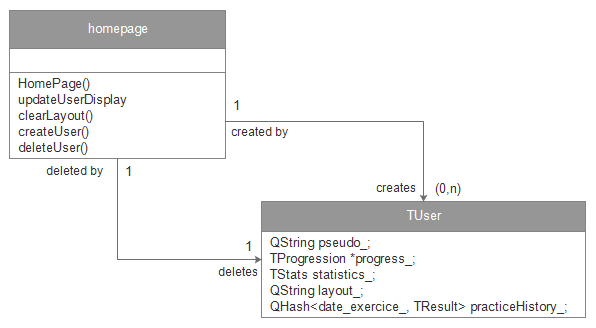
\includegraphics[width=12cm]{diagrams/Rhomepage.png}
	\caption{Relationship diagram for Home page}
	\label{Rhomepage} 
\end{figure}
\begin{figure}[H]
	\centering
	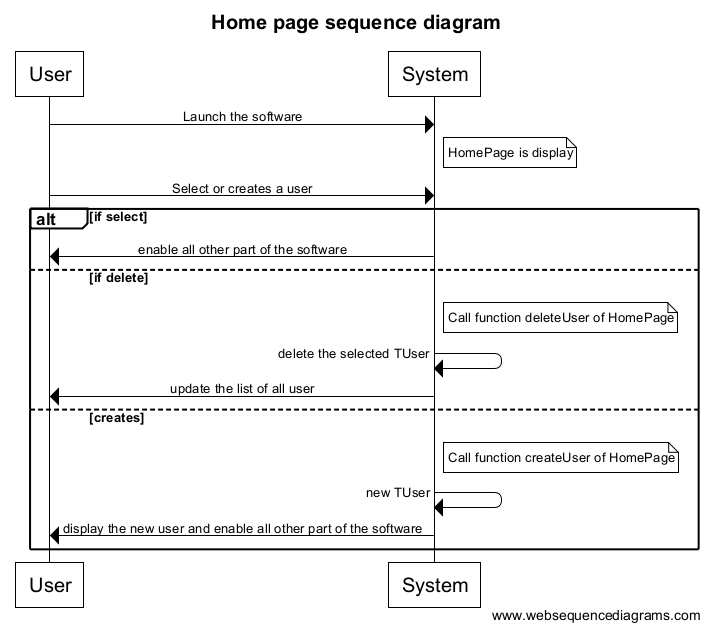
\includegraphics[width=12cm]{diagrams/Shomepage.png}
	\caption{Sequence diagram for Home page}
	\label{Shomepage}
\end{figure}
\begin{figure}[H]
	\centering
	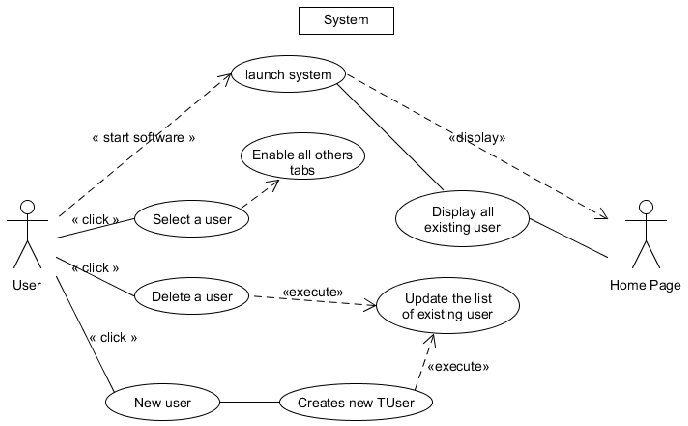
\includegraphics[width=12cm]{diagrams/UChomepage.png}
	\caption{User case diagram for Home page}
	\label{UChomepage}
\end{figure}

Next figures respectively show the relationship diagram (figure \ref{Rlearnpage}), the sequence diagram (figure \ref{Slearnpage}) and the Use Case diagram (figure \ref{UClearnpage}) (without details) for the learn page. Basically, the learn page works like this:
\begin{itemize}
\item The user has already started the software and selected a user.
\item The system shows all learning exercises to the user (including those already done and yet to be done exercises).
\item The user selects the exercises they want and the system display the corresponding one in a new window.
\item When the exercise is done the system shows the results to the user.
\end{itemize}

\begin{figure}[H]
	\centering
	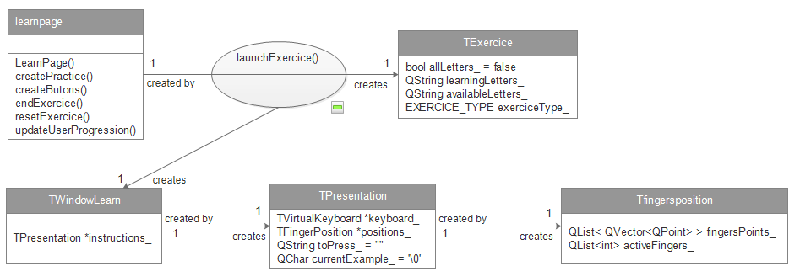
\includegraphics[width=12cm]{diagrams/Rlearnpage.png}
	\caption{Relationship diagram for Learn page}	
	\label{Rlearnpage}
\end{figure}
\begin{figure}[H]
	\centering
	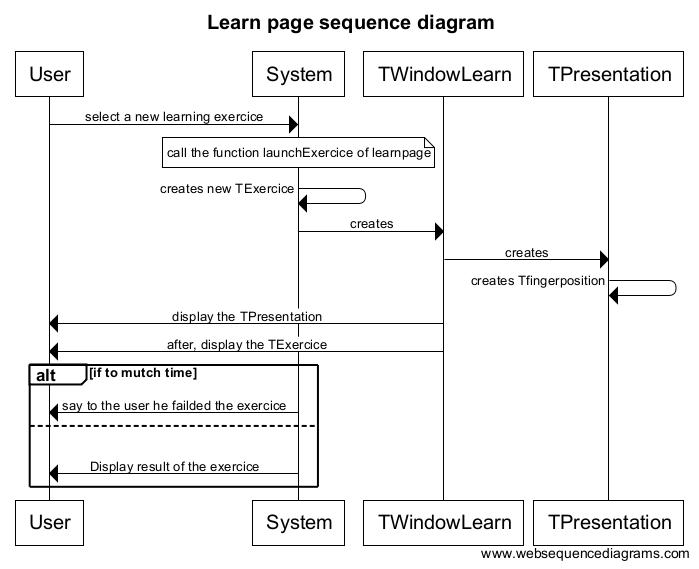
\includegraphics[width=12cm]{diagrams/Slearnpage.png}
	\caption{Sequence diagram for Learn page}
	\label{Slearnpage}
\end{figure}
\begin{figure}[H]
	\centering
	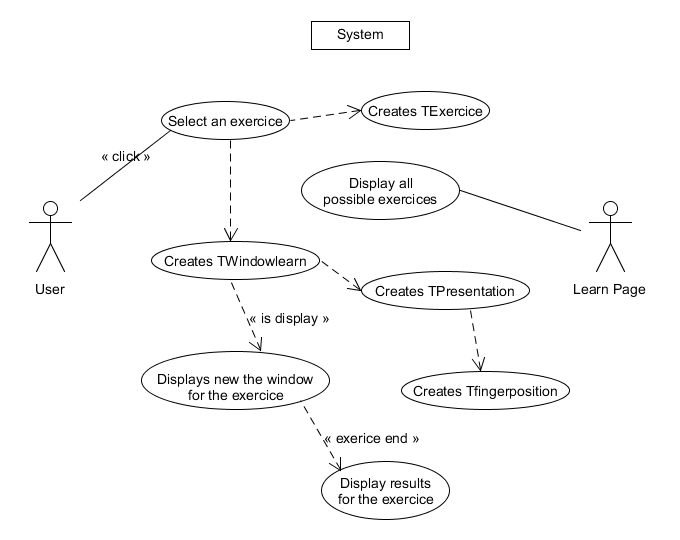
\includegraphics[width=12cm]{diagrams/UClearnpage.png}
	\caption{User case diagram for Leran page}
	\label{UClearnpage}
\end{figure}

Next figures respectively show the relationship diagram (figure\ref{Rpracticepage}), the sequence diagram (figure\ref{Spracticepage}) and the Use Case diagram (without details) for the practice page. Basically, the practice page works like this:
\begin{itemize}
\item The user has already started the software and selected a user.
\item The system shows all the four different exercises to the user.
\item The user selects the one they want and the system will display it in a new window.
\item When the exercise is done the system shows the results to the user.
\end{itemize}

\begin{figure}[H]
	\centering
    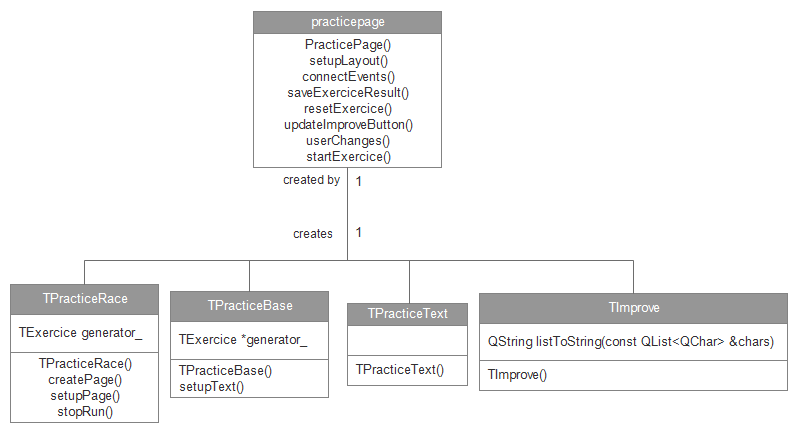
\includegraphics[width=12cm]{diagrams/Rpracticepage.png}
    \caption{Relationship diagram for Practice page}  
    \label{Rpracticepage} 
\end{figure}
\begin{figure}[H]
	\centering
    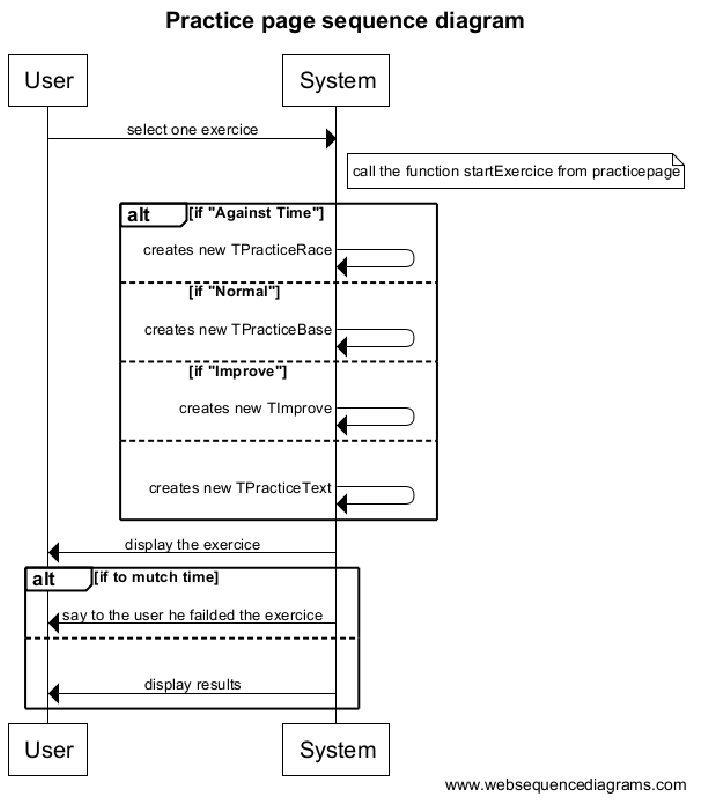
\includegraphics[width=12cm]{diagrams/Spracticepage.png}
    \caption{Sequence diagram for Practice page}
    \label{Spracticepage}
\end{figure}
\begin{figure}[H]
	\centering
    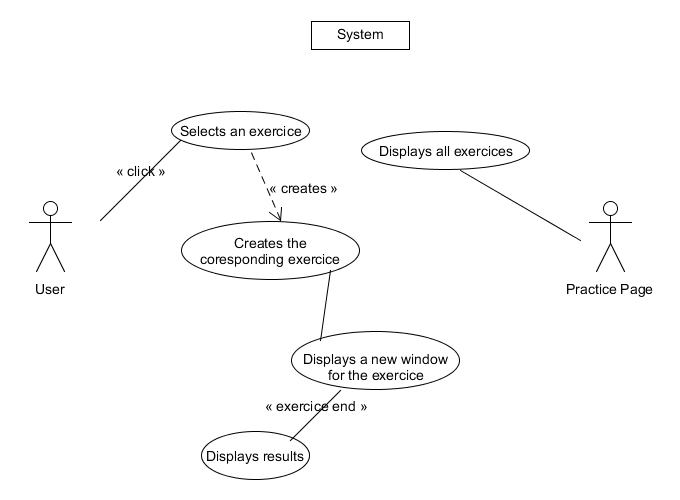
\includegraphics[width=12cm]{diagrams/UCpracticepage.png}
    \caption{User case diagram for Practice page}
    \label{UCpracticepage}
\end{figure}

Next figures respectively show the relationship diagram (figure\ref{Rgamepage}), the sequence diagram (figure\ref{Sgamepage}) and the Use Case diagram (without details) (figure\ref{UCgamepage}) for the game page. Basically, the game page works like this:
\begin{itemize}
\item The user has already started the software and selected a user.
\item Actually there is just one button in the game page so when the user clicks on it(or on a future one), the system starts the appropriate game in a new window.
\end{itemize}

\begin{figure}[h]
	\centering
    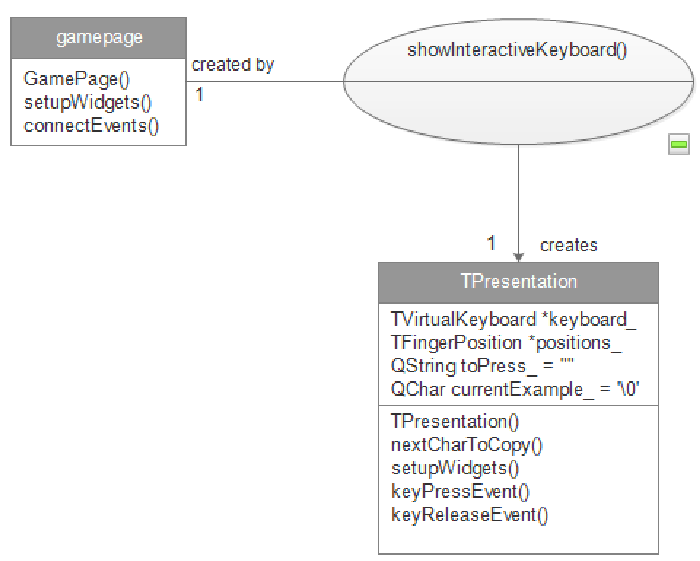
\includegraphics[width=12cm]{diagrams/Rgamepage.png}
    \caption{Relationship diagram for Game page}
    \label{Rgamepage}   
\end{figure}
\begin{figure}[h]
	\centering
    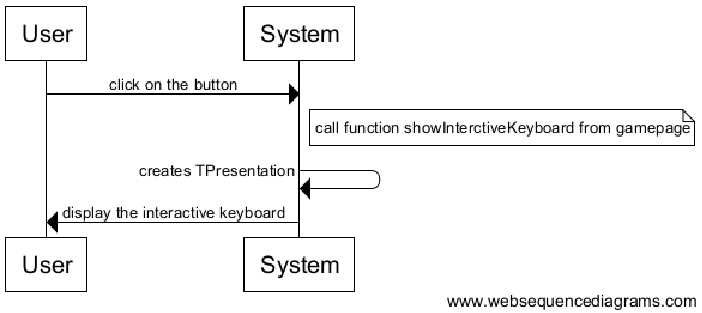
\includegraphics[width=12cm]{diagrams/Sgamepage.png}
    \caption{Sequence diagram for Game page}
    \label{Sgamepage}
\end{figure}
\begin{figure}[h]
	\centering
    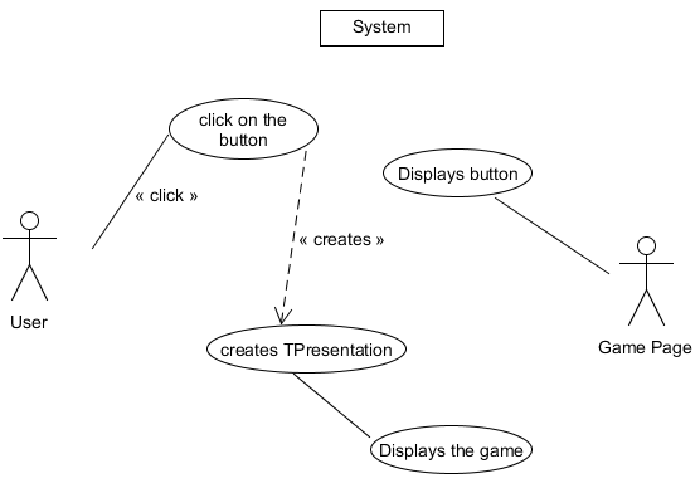
\includegraphics[width=12cm]{diagrams/UCgamepage.png}
    \caption{User case diagram for Game page}
    \label{UCgamepage}
\end{figure}

%------------------------------------
% Fin Partie Pierre
%------------------------------------
